% -*- mode: LaTeX; compile-command: "./build.sh" -*-

\documentclass[xcolor={usenames,dvipsnames,svgnames,table},12pt]{beamer}

\mode<presentation>
{
  \usetheme{default}                          % use a default (plain) theme

  \setbeamertemplate{navigation symbols}{}    % don't show navigation
                                              % buttons along the
                                              % bottom
  \setbeamerfont{normal text}{family=\sffamily}

%  \setbeamertemplate{footline}[frame number]

  \AtBeginSection[]
  {
    \begin{frame}<beamer>
      \frametitle{}
      \begin{center}
        {\Huge \insertsectionhead}

        \vspace{0.25in}
        \includegraphics[width=2in]{\secimage}
      \end{center}
    \end{frame}
  }
}

\newenvironment{xframe}[1][]
  {\begin{frame}[fragile,environment=xframe,#1]}
  {\end{frame}}

% uncomment me to get 4 slides per page for printing
% \usepackage{pgfpages}
% \pgfpagesuselayout{4 on 1}[uspaper, border shrink=5mm]

% \setbeameroption{show only notes}

\usepackage[english]{babel}
\usepackage[T1]{fontenc}
\usepackage{graphicx}
\graphicspath{{images/}}

\usepackage{ulem}
\usepackage{url}
\usepackage{fancyvrb}

\usepackage[backend=pgf, input, extension=pgf, outputdir=diagrams]{diagrams-latex}

\usepackage{minted}

% TODO: include picture of Fenwick tree on title slide

\title{You Could Have Invented Fenwick Trees!}
\date{
\includegraphics[height=0.25in]{plclub-logo_small} \\ 21 May 2021}
\author{Brent Yorgey}

%%%%%%%%%%%%%%%%%%%%%%%%%%%%%%%%%%%%%%%%%%%%%%%%%%%%%%%%%%%%%%%%%%%

\begin{document}

\maketitle

\begin{frame}{About me}
  \begin{center}
  \raisebox{-0.25\height}{
\includegraphics[height=0.25in]{plclub-logo_small}} (2008--2014) \\[0.25in]
  \raisebox{-0.25\height}{
\includegraphics[height=0.25in]{HENDRIX_LOGO_RGB}} (2015--) \\[0.25in]

  Things I Like (a very small sample):\\
  FP, EDSLs, combinatorics, category theory,
  teaching, competitive programming, questions from the audience
  \end{center}
\end{frame}

\begin{frame}{About this talk}
  TODO: graph of git commits on this project
\end{frame}

% TODO: drawArray a_1 ... a_8 as section image
\def\secimage{plclub-logo_small}
\section{Introduction}

\begin{xframe}{Sequence operations}
\begin{center}
\begin{diagram}[width=150]
import FenwickDiagrams

dia = vsep 0.5
  [ drawArray (draw . ("a_"++) . show) [1 :: Int .. 8]
  , mconcat
    [ arrowV unit_Y
    , text "update" # fontSizeL 0.5 # translate (1.5 ^& (-0.5))
    ]
    # translateX (3*leafWidth)
  , drawArray draw2 [1 :: Int .. 8]
  , rangeBracket 2 5
  , mconcat
    [ arrowV unit_Y
    , text "range query" # fontSizeL 0.5 # translate (2.2 ^& (-0.5))
    ]
    # translateX (2.5 * leafWidth)
  , text "$a_2 + a_3 + x + a_5$" # fontSizeL 0.6
    # translateX (2.5 * leafWidth)
  ]
  where
    draw2 4 = draw "x"
    draw2 n = draw ("a_" ++ show n)
\end{diagram}
\end{center}
\end{xframe}

% IFTIME: use colors for ranges instead of brackets
\begin{xframe}{Prefix queries}
\begin{center}
\begin{diagram}[width=150]
import FenwickDiagrams

dia = vsep 0.5
  [ drawArray draw (map (("a_"++) . show) [1 :: Int .. 8])
  , rangeBracket 3 6
  , text "=" # translateX (3.5 * leafWidth) <> strutY 1
  , drawArray draw (map (("a_"++) . show) [1 :: Int .. 8])
  , rangeBracket 1 6
  , text "-" # translateX (3.5 * leafWidth) <> strutY 1
  , drawArray draw (map (("a_"++) . show) [1 :: Int .. 8])
  , rangeBracket 1 2
  ]
  # fontSizeL 0.7
\end{diagram}
\end{center}
\end{xframe}

\begin{xframe}{Solutions}
  \begin{center}
  \begin{tabular}{ccc}
    approach & update & prefix query \\
    \onslide<2->{just store sequence} & $O(1)$ & $O(n)$ \\
    \onslide<3->{cache prefix sums}    & $O(n)$ & $O(1)$ \\
    \onslide<4->{cache more cleverly\dots?} & $O(\lg n)$ & $O(\lg n)$
  \end{tabular}
  \end{center}
\end{xframe}

\begin{xframe}{Segment trees}
\begin{center}
\begin{diagram}[width=300]
  import FenwickDiagrams
  import SegTree

  dia :: Diagram B
  dia = sampleArray
    # mkSegTree
    # fmap getSum
    # drawSegTree def
\end{diagram}

(assume $n = 2^k$)
\end{center}
\end{xframe}

\begin{xframe}{Updating a segment tree}
\begin{center}
\begin{diagram}[width=300]
  import FenwickDiagrams
  import SegTree
  import Data.Monoid
  import Control.Arrow ((***))

  dia :: Diagram B
  dia = sampleArray
    # map ((,) (Any False))
    # mkSegTree
    # update 5 (Any True, Sum 3)
    # fmap (getAny *** getSum)
    # drawSegTree (mkSTOpts showUpdateOpts)
\end{diagram}
\end{center}
\end{xframe}

\begin{xframe}{Range query on a segment tree}
\begin{center}
\begin{diagram}[width=300]
  import FenwickDiagrams
  import SegTree
  import Data.Monoid
  import Control.Arrow ((***), second)

  dia :: Diagram B
  dia = vsep 0.7
    [ sampleArray
      # mkSegTree
      # rq' i j
      # fst
      # drawSegTree (mkSTOpts showRangeOpts)
    , (fst (leafX i n) ^& 0) ~~ (snd (leafX j n) ^& 0)
      # lc green
      # applyStyle defRangeStyle
    ]
    where
      i = 4
      j = 11
      n = length sampleArray
\end{diagram}
\end{center}
\end{xframe}

% TODO: get rid of range bars in this diagram
\begin{xframe}{Thinning segment trees}
\begin{center}
\begin{diagram}[width=300]
  import FenwickDiagrams
  import SegTree
  import Data.Monoid
  import Control.Arrow ((***), first, second)

  dia :: Diagram B
  dia = sampleArray
    # mkSegTree
    # fmap getSum
    # drawSegTree def
\end{diagram}
\end{center}
\end{xframe}

\begin{xframe}{Thinning segment trees}
\begin{center}
\begin{diagram}[width=300]
  import FenwickDiagrams
  import SegTree
  import Data.Monoid
  import Control.Arrow ((***), first, second)

  dia :: Diagram B
  dia = sampleArray
    # mkSegTree
    # deactivate
    # drawSegTree (mkSTOpts (showInactiveOpts False))
\end{diagram}
\end{center}
\end{xframe}

% TODO: picture showing how any prefix corresponds to a specific
% collection of active nodes?

\begin{xframe}{Storing a thinned segment tree}
\begin{center}
\begin{diagram}[width=300]
  import FenwickDiagrams
  import SegTree
  import Data.Monoid
  import Control.Arrow ((***), first, second)

  dia :: Diagram B
  dia = vsep 0.5
    [ sampleArray
      # mkSegTree
      # deactivate
      # drawSegTree opts
    , arrowV (2 *^ unit_Y)
    , sampleArray
    # mkFenwickArray
    # drawArray (draw . getSum)
    # centerX
    ]

  opts = (mkSTOpts (showInactiveOpts False))
    { drawEdge = drawSlidingEdges }
\end{diagram}
\end{center}
\end{xframe}

% TODO include range bars in this picture

\begin{xframe}{Fenwick tree = right-leaning, thinned segment tree}
  \begin{center}
\begin{diagram}[width=300]
import FenwickDiagrams
import SegTree

dia :: Diagram B
dia = sampleArray
  # mkSegTree
  # deactivate
  # drawSegTree stOpts

stOpts = (mkSTOpts nOpts)
  { leanRight = True }

nOpts = (showInactiveOpts False)
  { leanRightN = True }
\end{diagram}

\onslide<2>{\dots but how to move around?}
  \end{center}
\end{xframe}

\begin{xframe}{Fenwick trees}
  \begin{center}
    \begin{minipage}{0.45\textwidth}
      \raisebox{-0.5\height}{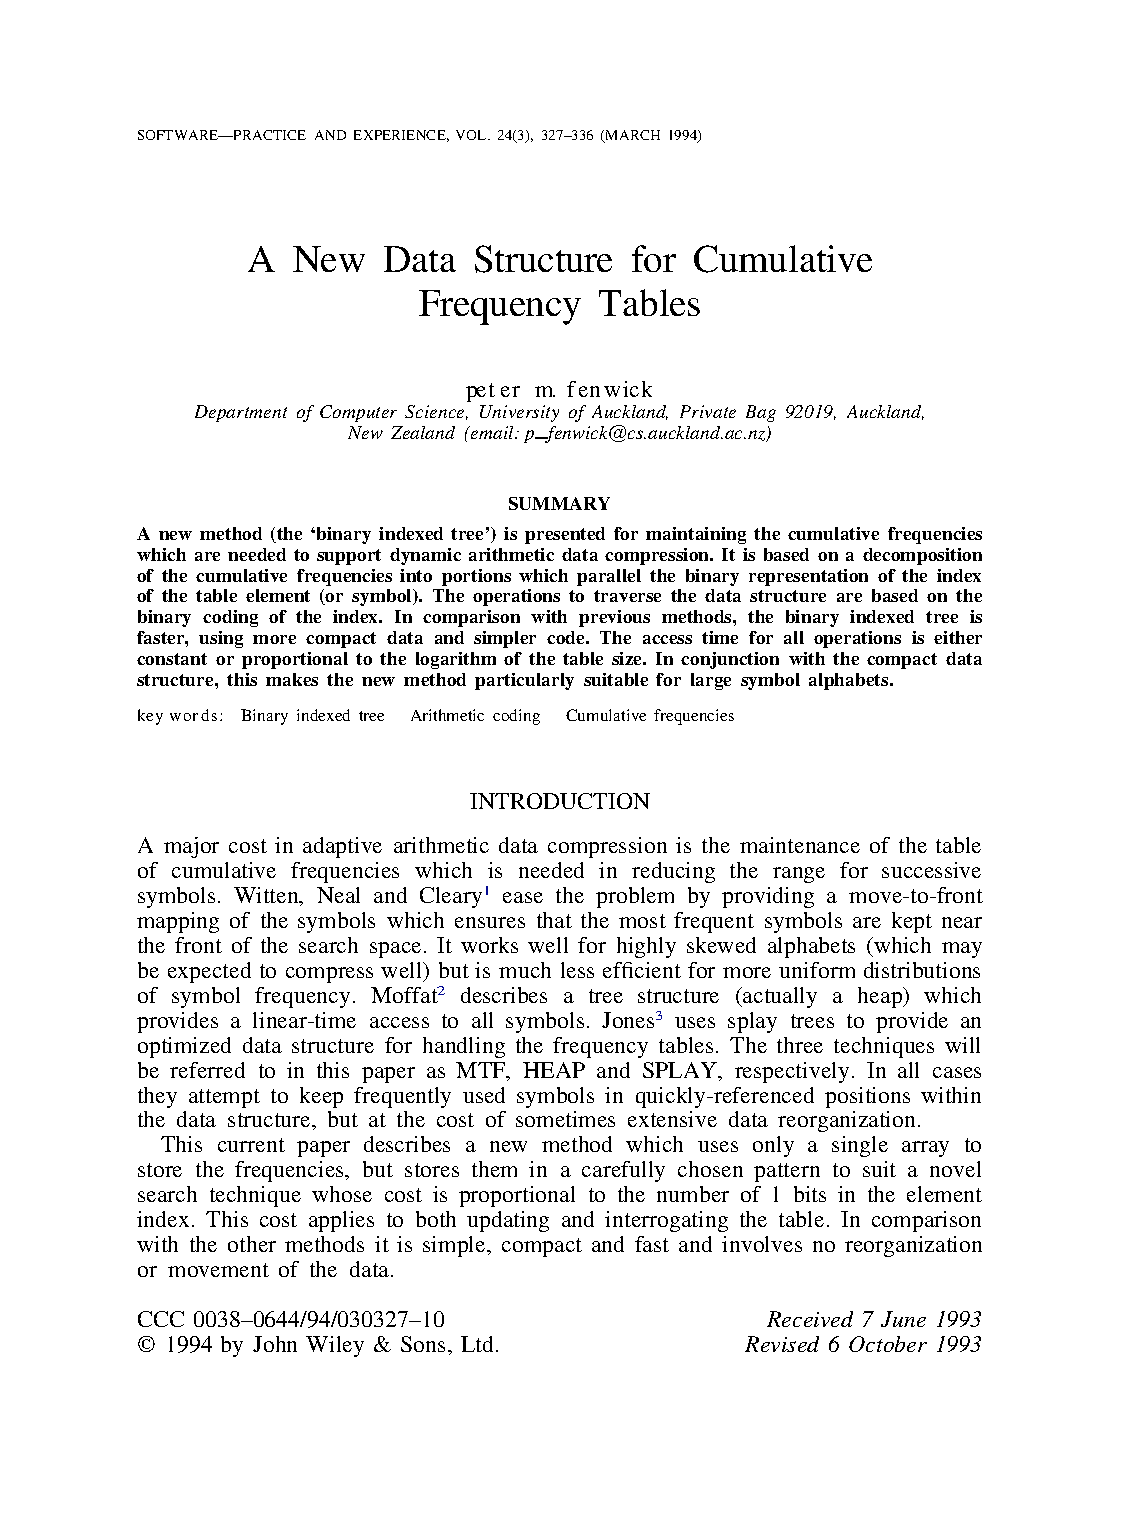
\includegraphics[height=3in]{fenwick-p1}}
    \end{minipage}
    \hspace{0.25in}
    \begin{minipage}{0.45\textwidth}
      Peter Fenwick, 1994 \\
      A New Data Structure for Cumulative Frequency Tables
    \end{minipage}
  \end{center}
\end{xframe}

\begin{xframe}{Fenwick trees}
  % TODO: show Ryabko paper?
\end{xframe}

\begin{xframe}{XXX}
  
  \inputminted{java}{Fenwick.java}
\end{xframe}

\end{document}
